\documentclass[%
  a4paper,oneside,%
  %arial,
  11pt,% <10pt, 9pt>
  smallchapters,
  %style=screen,
  %sender=bottom,
  green,% <orange, green, violet>
  rgb, <cmyk>
  %mono
  ,]{tubsbook}
  
\usepackage{listings}  % for code stuff
\usepackage{bm} 
 
\renewcommand{\familydefault}{\sfdefault}
\usepackage[utf8]{inputenc}
\RequirePackage{scrlfile}
\ReplacePackage{scrpage2}{scrlayer-scrpage}

\usepackage[ngerman,english]{babel}

\usepackage{lipsum} % Blindtext-Paket
\definecolor{InAGreen}{RGB}{172,193,58}

% Titelseiten-Elemente
\title{A Statistical Approach for the Fusion of Data and
Finite Element Analysis in Vibroacoustics}
\subtitle{Untertitel}
\author{Lucas Hermann}
%\logo{Institut fuer Lorem Ipsum}
\logo{
\includegraphics{InA-Logo-rgb.pdf}}
\titleabstract{\lipsum[2]}
\titlepicture{infozentrum.jpg}
% Rückseiten-Elemente
\address{%
  Herr Mustermann\\
  Schlossallee 1\\
  33333 Darmstadt}
\backpageinfo{%
  \lipsum[5]
}
\usepackage{pdfpages}								% Einbinden von PDF-Pages
\usepackage[colorlinks,pdfpagelabels,pdfstartview = FitH,bookmarksopen = true,bookmarksnumbered = true,linkcolor = black,plainpages = false,hypertexnames = false,citecolor = black] {hyperref}
\usepackage[figure]{hypcap} 
\bibliographystyle{ieeetr}

\begin{document}

%\maketitle[image,logo=left]%[<plain/image/imagetext>,<logo=left/right>]
%\makebackpage[trisec]%[<plain/info/addressinfo>]
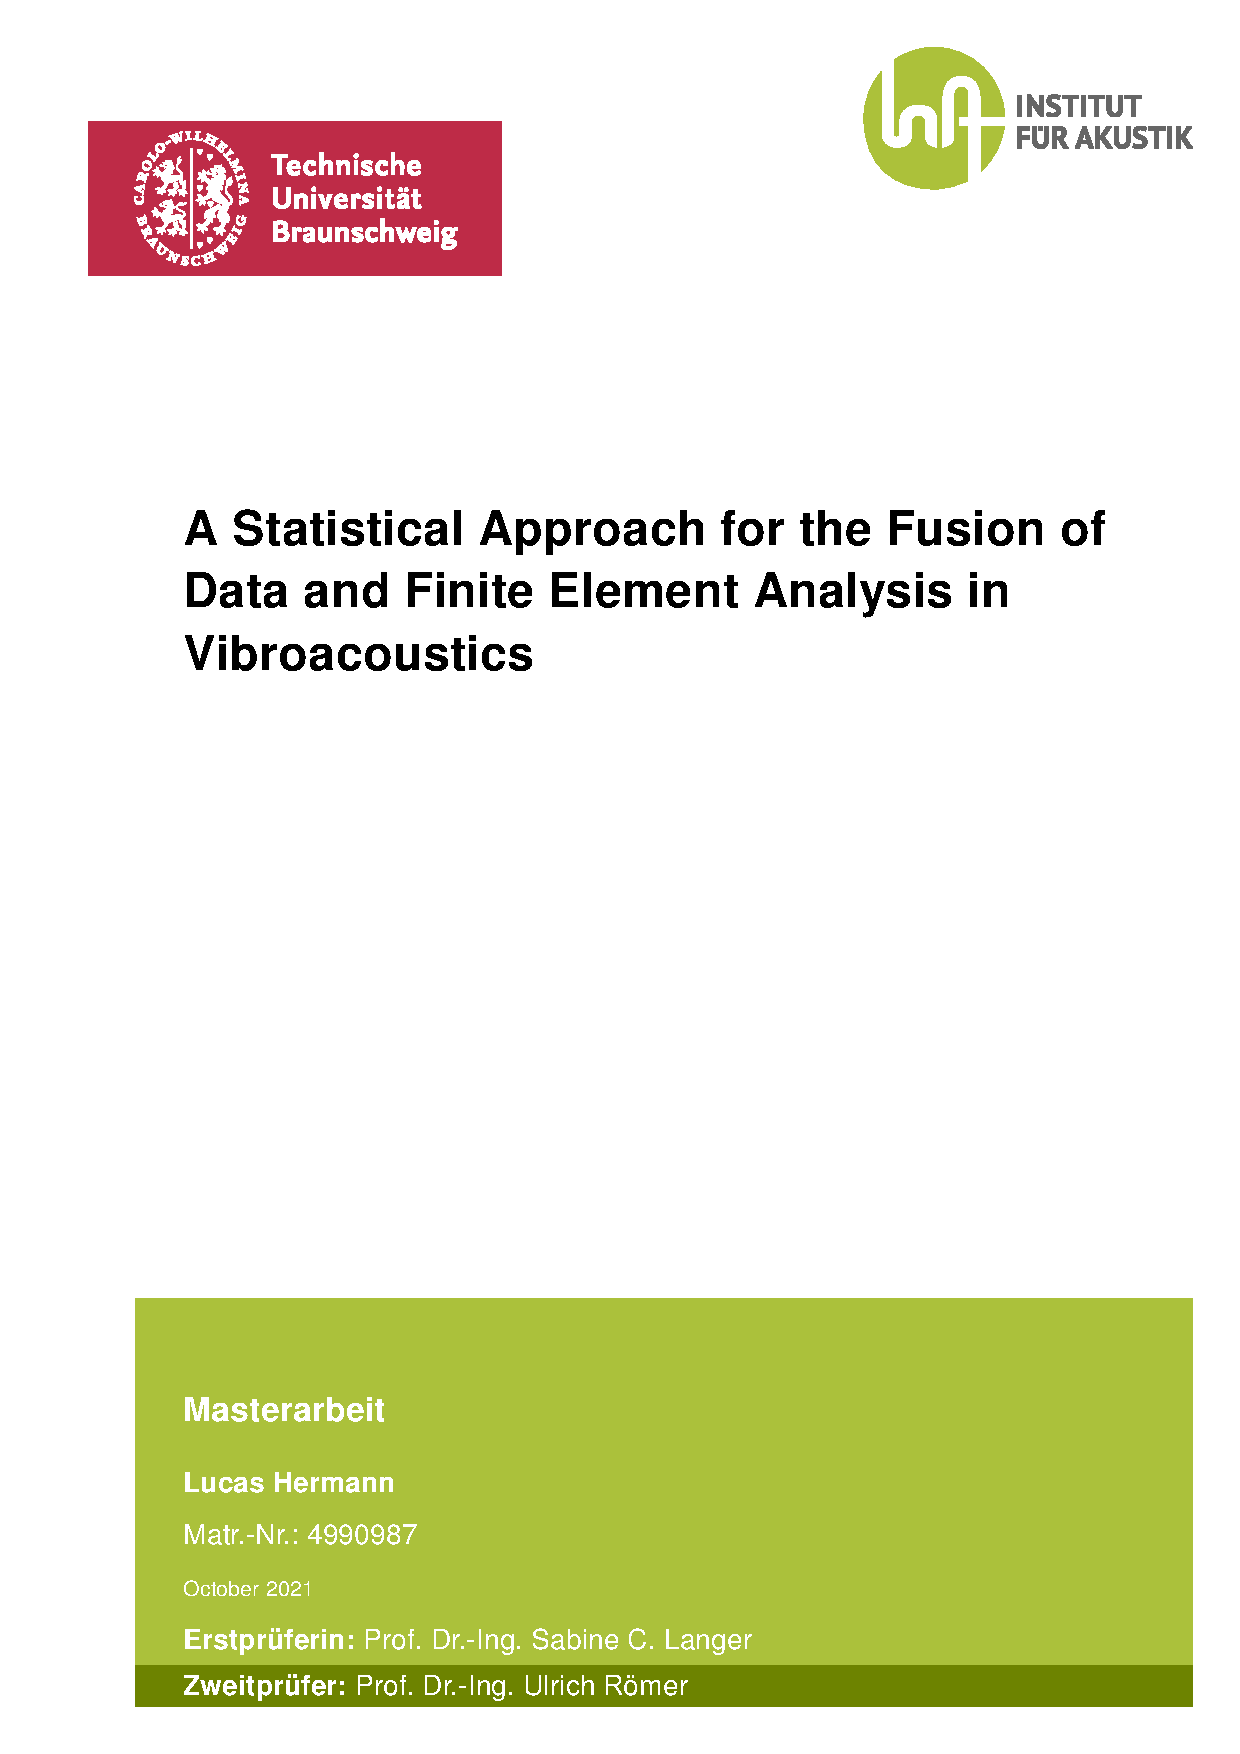
\includepdf[pages=-]{./Deckblatt/2099_StA_Name_Deckblatt.pdf}

\chapter*{Declaration}
Hiermit versichere ich, Lucas Hermann, durch meine Unterschrift, dass ich die
vorliegende Masterarbeit mit dem Titel ``<<Titel>>'' selbständig und ohne Benutzung
anderer als der angegebenen Hilfsmittel angefertigt habe. Alle Stellen, die wörtlich oder sinn-
gemäß aus veröffentlichten oder unveröffentlichten Schriften entnommen sind, habe ich als
solche kenntlich gemacht. Insbesondere sind auch solche Inhalte gekennzeichnet, die von
betreuenden wissenschaftlichen Mitarbeiterinnen und Mitarbeitern des Instituts für Akustik eingebracht wurden.

Die Arbeit oder Auszüge daraus haben noch nicht in gleicher oder ähnlicher Form dieser
oder einer anderen Prüfungsbehörde vorgelegen.

Mir ist bewusst, dass Verstöße gegen die Grundsätze der Selbstständigkeit als Täuschung
betrachtet und entsprechend der Prüfungsordnung geahndet werden.

\begin{flushright}
Braunschweig, \today
\end{flushright}

\vspace{2cm}
\hspace{2cm}\rule{5cm}{1pt}

\hspace{2cm}\small{Lucas Hermann} 

\chapter*{Abstract}
\lipsum[1]

\tableofcontents


\chapter{Introduction}

\textcolor{tubsSecondary}{Dies ist ein Text in \texttt{tubsSecondary}.}
\textcolor{tubsViolet}{Dies ist ein Text in \texttt{tubsViolet}.}
\textcolor{tubsGreenDark}{Dies ist ein Text in \texttt{tubsGreenDark}.}\bigskip

\lipsum[1]

\begin{itemize}
  \item Aufzählungspunkt Eins
  \item Aufzählungspunkt Zwei
    \begin{itemize}
      \item Unter-Aufzählungspunkt Eins
      \item Unter-Aufzählungspunkt Zwei
    \end{itemize}
  \item Aufzählungspunkt Drei
\end{itemize}

\chapter{Theoretical Background}

\section{The Classical Finite Element Method}

\section{Bayesian Inference}
$posterior = \frac{likelihood x prior}{marginal likelihood}$ (Rasmussen p.9)


\section{Gaussian Process Regression}
Gaussian Processes are a class of Bayesian non-parametric models. Non-parametric doesn't mean that there are no parameters involved but rather that there is an infinite number of them. Every realization of a Gaussian process doesn't yield a scalar or vector but a function. One can think of a Gaussian Process as a collection of infinitely many normally distributed random variables, i.e. a generalization of a Gaussian distribution: A vector with infinitely many entries is basically a function. By picking out a finite set of those random variables when discretizing e.g. on an FEM mesh, one obtains a multivariate distribution which is determined by a mean and a covariance matrix. [Rasmussen p.2] Hence, the GP assigns a confidence band to a function where a usual parametric regression wouldn't.

-Regression in general
-differences of a GP regression to e.g. a polynomial regression: every point is assgined an uncertainty

-Herleitung der Kovarianzmatrix, evtl. auch für das standard linear regression modell


\subsection{Prior before observation}

\subsection{Posterior after observation}

\section{The Statistical Finite Element Method}
The differential equation is treated from a Bayesian viewpoint: all parameters are random variables. For dependent parameters not a single distribution but a Gaussian Process is applied. Therefore prior to solving the FEM linear system, the parameter $GP f(x)$ is sampled. That sample is evaluated for each cell in the FEM mesh which makes it necessary to assemble the system matrix with that in mind.

\subsection{Probabilistic FEM Prior}
The prior before observation is obtained by computing the FEM response $u_h$ of the PDE given all parameters. The random parameters are modeled as GPs. Thereby result a mean $\bar{u_h}$ and a covariance matrix $C_u$. For this being the prior, the GP hyperparameters are chosen deterministically. The covariance matrix is obtained by calculating $C_u = A^{-1} C_{par} A^{-T}$ with $A$ the FEM system matrix and $C_{par}$ the covariance matrix of the respective random parameter's GP. The mean can easily be determined by calculating the deterministic mean of the FEM by using only the GP's mean.
The resulting response $u_h$ is, since it is discretized and not continuous, a multivariate Gaussian distribution.
%
To check convergence of the FEM model, it can be compared to the exact analytically determined system response $u$. 
%
It is assumed that there is a difference between the exact and the calculated FEM response to the true system response. That difference ought to be reduced by updating the prior with observations.


\subsection{Inference of the Posterior Density}
To infer the posterior density, observed data is necessary. These can be obtained by either actually measuring a physical process or by generating synthetic data which allows developing and improving the statFEM model already before having to set up an experiment and take real measurements beforehand.
%
Sampling from a synthetic source or from the real physical response yields the observation vector
%
\begin{equation}
\bm{y} = {z} + {e}
\end{equation}
%
with $z$ the real response and $e$ the measurement error which is also a part of $\bm{y}$ for the synthetic observations. It can be seen that the model mismatch error $\bm{d}$ is, as opposed to eq. (), not part of the equation because it is only part of the FEM modeling error. 
%
The data is observed on multiple measurement  points $n_y$ throughout the domain. It can be chosen if the data is assumed to be deterministic or to be random. For the deterministic case only one value is measured for each measurement point. In the random case many measurements are taken per point what leads to a probability distribution for each point.
%
Now, Bayes' rule can be applied to update the prior with the observations.
The result of this operation is
%
\begin{equation}
p(u|y) = \mathcal{N}(\bar{u_{|y}}, C_{u|y})
\end{equation}
%
with
%
\begin{equation}
\bar{u_{|y}} = C_{u|y} \left(   \rho P^T  (C_d + C_e)^{-1}  y  +  C_u^{-1}  \bar{u}   \right)
\end{equation}
and
\begin{equation}
C_{u|y} = \left(      \rho^2  P^T   (C_d + C_e)^{-1}  P  +  C_u^{-1}    \right)^{-1}
\end{equation}

\chapter{1D Example and Application in Vibroacoustics}

\section{Simple 1D example}
\paragraph{Choice of PDE}
The Poisson equation 
%%
\begin{equation}
- \nabla \cdot \mu(x) \nabla u(x) = f(x)
\label{eqn:Poisson}
\end{equation}
%%
is chosen as the governing equation. It is an elliptic partial differential equation (PDE). In this work it is used as a simple 1D example to illustrate how the statistical FEM and especially the Gaussian Process Regression works.
The most standard form of it does not, contrary to this example, include $\mu(x) \in \mathbb{R}^+$ which is the diffusion coefficient dependent on the spatial variable $x$. The right-hand side consists of the source term $f(x)\in \mathbb{R}$. Both $\mu (x)$ and $f(x)$ are the free parameters in this case. The equation is solved for the unknown  $u(x)$ in the domain $\Omega = (0,1)$ with the boundary condition $u(x) = 0$ on $x=0$ and $x=1$.
%
For a first example there holds $\mu(x)=1$. $f(x)$ is modeled as a Gaussian Process [Cirak]
%
\begin{equation}
f(\bm{x}) \sim \mathcal{GP} \left( \bar{f}(\bm{x}), c_f(\bm{x},\bm{x}')\right) \;.
\end{equation}
%
\paragraph{Construction of the GP}
The mean function of the GP is set to $\bar{f}(x) = 1.0$. For the covariance function at first a squared exponential kernel 
%
\begin{equation}
c_f(\bm{x},\bm{x}') =    \sigma_{f}^2 \exp \left(-  \frac{\left \| \bm{x}-{\bm{x}}' \right \|^2}{2l_{f}^2} \right )       
\label{eqn:sqEx_f}
\end{equation}
%
is used with the standard deviation $\sigma_{f} = 0.1$ and the length scale $l_{f} = 0.4$.
In Python the kernel is directly implemented as a function which takes two lists and the parameters as input variables [Murphy]:
\begin{lstlisting}[language=Python]
def squared_exponential(xa, xb, lf, sigf):
    sq_norm = -0.5 * scipy.spatial.distance.cdist(xa, xb, 'sqeuclidean') \
    	* (1/lf**2)
    return sigf**2 * np.exp(sq_norm) .
\end{lstlisting}
\label{lst:sqEx}
%
Here, the parameters are fixed but in a later example a method on how to infer the optimum position for these will be studied.

Having prepared the mean function and the kernel, which can be considered the prior in a GP regression setting, a sample of the GP can be drawn. For this points have to be chosen on which the kernel is evaluated. These are the test points and, according to [Cirak], correspond to the center of the FEM cells. This implies that there are as many test points as FEM cells and therefore the coordinates of the FEM mesh can directly be used to compute the covariance matrix. For that (\ref{eqn:sqEx_f}) is evaluated at $\bm{x} = \bm{x}'$ with $\bm{x}$ the vector of test points. 

A GP has the marginalization property: if you sample it at a finite number of points it yields a multivariate Gaussian distribution $\mathcal{N}(\bar{\bm{f}},\bm{C_f})$ with $\bar{\bm{f}}$ the mean vector and $\bm{C_f}$ the covariance matrix while still describing the underlying continuous sample.
According to [Rasmussen] sampling from a multivariate Gaussian distribution works as follows: To obtain $n$ samples from the prior, at first $n$ samples of a standard normal distribution, also called Gaussian white noise, $e \sim \mathcal{N}(0,1)$ have to be drawn. Computing the Cholesky decomposition of the covariance matrix $\bm{C_f} = LL^T$, which can also be thought of as taking the square root of a matrix, yields the lower triangular matrix $L$. Samples can now easily be drawn from $\bm{f} = \bar{\bm{f}} + Le$ which is a multivariate Gaussian distribution with a mean $\bm{f}$ and a covariance $\bm{C_f}$.

Sample: Normal distribution times std dev. GP with n points is basically a multivariate gaussian with n dimensions. therefore we need the std dev. for a univariate gaussian thats . 

For the observations made in a later step it is assumed that there is some measurement noise. This is modeled as an added variance $\sigma_{n}^2$ on the diagonal of the prior covariance matrix. An additional effect of this added noise is the improved numerical stability of the covariance matrix which is important for computing the Cholesky decomposition.

\section{1D Vibroacoustics Example}
Helmholtz Equation. Looks similar to the Poisson equation but the right side differs. It's the eigenvalue problem for the laplace operator.

\lipsum[2-5] %\cite{campolina}



\chapter{Results and Discussion}

\lipsum[1-3] %\cite{Langer2019}

\section{Section 1}

\lipsum[4-7] %\cite{Yaghoubi:2017}


\begin{thebibliography}{4}
%
\bibitem{campolina}
Campolina, B.: Vibroacoustic modelling of aircraft double-walls with structural links using Statistical
Energy Analysis (SEA). Acoustics [physics.class-ph]. Université de Sherbrooke; Université Pierre
et Marie Curie - Paris VI (2012)

\bibitem{Langer2019}
Langer, S.C., Blech, C.: Cabin noise prediction using wave‐resolving aircraft models. Proc. Appl. Math. Mech., Vol. 12 (1) (2019): e201900388. doi:10.1002/pamm.201900388

\bibitem {Yaghoubi:2017} Yaghoubi, V., Marelli, S., Sudret, B., Abrahamsson, T.: Sparse polynomial chaos expansions of frequency response functions using stochastic frequency transformation, Probabilistic Engineering Mechanics, volume 48, pages 39-58 (2017)
\end{thebibliography}

\end{document}
